\documentclass[12pt,a4paper]{article}

% 中文支持
\usepackage[UTF8]{ctex}
\usepackage{geometry}
\geometry{left=2.5cm,right=2.5cm,top=2.5cm,bottom=2.5cm,headheight=14.5pt}

\usepackage{amsmath,amssymb}
\usepackage{graphicx}
\usepackage{booktabs}
\usepackage{multirow}
\usepackage{xcolor}
\usepackage{hyperref}
\usepackage{listings}
\usepackage{float}
\usepackage{caption}
\usepackage{subcaption}
\usepackage{enumitem}
\usepackage{fancyhdr}
\usepackage{titlesec}

\hypersetup{
    colorlinks=true,
    linkcolor=blue,
    citecolor=blue,
    urlcolor=blue,
}

\lstset{
    language=Python,
    basicstyle=\ttfamily\small,
    keywordstyle=\color{blue},
    stringstyle=\color{red},
    commentstyle=\color{gray},
    numbers=left,
    numberstyle=\tiny\color{gray},
    stepnumber=1,
    numbersep=5pt,
    backgroundcolor=\color{white},
    frame=single,
    framerule=0.5pt,
    breaklines=true,
    showstringspaces=false,
    tabsize=4,
    captionpos=b,
}

\pagestyle{fancy}
\fancyhf{}
\fancyhead[C]{基于SigLIP的小规模图文检索系统——最终报告}
\fancyfoot[C]{\thepage}

\title{\textbf{基于SigLIP的小规模图文检索系统}\\\Large 最终报告}
\author{Yi Kai}
\date{2026年5月}

\begin{document}

\maketitle
\thispagestyle{fancy}

\begin{abstract}
本项目基于 SigLIP（Sigmoid Loss for Language-Image Pretraining）模型，在 Flickr8k 数据集上实现了一个小规模图文检索系统。与 CLIP 使用 softmax 进行全局归一化不同，SigLIP 对每个图文对独立使用 sigmoid 判断是否匹配，对 batch size 更鲁棒。本文详细介绍了模型实现、训练优化过程、实验结果分析及可视化，最终最优模型（Exp6：ResNet18 width=48 + Transformer + ColorJitter + Cosine Warmup）在测试集上取得了 t2i\_R@1=36.65\%、i2t\_R@1=39.82\% 的检索准确率。
\end{abstract}

\tableofcontents
\newpage

%=======================================================================
\section{任务概述}
%=======================================================================

本项目基于 SigLIP 模型，在 Flickr8k 数据集上训练并评估一个图文检索系统。核心任务包括：

\begin{enumerate}[nosep]
    \item 理解 CLIP 与 SigLIP 在损失函数上的差异；
    \item 使用 PyTorch 实现图像编码器（ResNet18）、文本编码器（Transformer）和 SigLIP 损失函数；
    \item 在 Flickr8k 数据集上训练模型，报告 Text-to-Image 与 Image-to-Text 的 Recall@1/5/10；
    \item 分析模型在多模态语义对齐方面的效果并进行可视化；
    \item 基于 \texttt{google/siglip-base-patch16-224} 预训练模型体验图文交叉相似度矩阵可视化。
\end{enumerate}

Flickr8k 数据集包含 8000 张图像，每张配有 1--5 条英文描述，共约 40000 条图文对。数据划分为训练集（6000 张）、验证集（1000 张）和测试集（1000 张）。

%=======================================================================
\section{模型结构}
%=======================================================================

\subsection{图像编码器：ResNet18}

采用自定义 ResNet18 作为图像编码器，核心组件为 \texttt{BasicBlock}：

\begin{lstlisting}[caption={ResNet BasicBlock 实现}]
def __init__(self, in_channels, out_channels, stride=1, downsample=None):
    super().__init__()
    self.conv1 = nn.Conv2d(in_channels, out_channels,
                      kernel_size=3, stride=stride, padding=1, bias=False)
    self.bn1   = nn.BatchNorm2d(out_channels)
    self.conv2 = nn.Conv2d(out_channels, out_channels,
                    kernel_size=3, stride=1, padding=1, bias=False)
    self.bn2   = nn.BatchNorm2d(out_channels)
    self.relu  = nn.ReLU(inplace=True)
    self.downsample = downsample
\end{lstlisting}

残差连接逻辑为：
\[
\text{out} = \text{ReLU}(\text{BN}_2(\text{Conv}_2(\text{ReLU}(\text{BN}_1(\text{Conv}_1(x))))) + \text{identity})
\]

当主路改变了通道数或空间尺寸时，\texttt{downsample}（1$\times$1 卷积+BN）对齐捷径形状。

最终架构：4 层残差层（通道数 $[w, 2w, 4w, 8w]$，$w$ 为 base width），全局平均池化后接线性投影层映射到共享语义空间（维度 256）。最优配置使用 $w=48$。

\subsection{文本编码器：Transformer}

采用 2 层 Pre-LN Transformer 作为文本编码器：

\begin{lstlisting}[caption={Transformer 文本编码器 forward}]
def forward(self, input_ids):
    x = self.token_embedding(input_ids)          # [B, L, D]
    x = self.positional_encoding(x)               # 加位置编码
    padding_mask = input_ids.eq(self.padding_idx)  # True=忽略
    x = self.encoder(x, src_key_padding_mask=padding_mask)
    mask = (~padding_mask).unsqueeze(-1).float()
    x = (x * mask).sum(dim=1) / mask.sum(dim=1).clamp(min=1)  # 均值池化
    x = self.proj(x)                               # 线性投影
    return x
\end{lstlisting}

关键设计：均值池化时忽略 PAD 位置，仅对有效 token 做加权平均；4 头注意力（$D=256$，每头 64 维），FFN 隐藏维度 1024。

\subsection{SigLIP 损失函数}

SigLIP 与 CLIP 的核心区别在于损失函数：CLIP 使用 softmax 进行全局归一化（每个样本与 batch 内所有其他样本竞争），而 SigLIP 对每个图文对独立使用 sigmoid（二分类判断是否匹配）。

设一个 batch 中包含 $|\mathcal{B}|$ 个图文样本对，图像编码为 $\mathbf{v}_i$，文本编码为 $\mathbf{t}_j$，二者归一化后的余弦相似度为：
\[
z_{ij} = \frac{\mathbf{v}_i \cdot \mathbf{t}_j}{\|\mathbf{v}_i\| \|\mathbf{t}_j\|}
\]

引入可学习温度系数 $t = \exp(\log t)$ 和偏置项 $b$，定义缩放 logits：
\[
\ell_{ij} = t \cdot z_{ij} + b
\]

匹配标签定义为对角线 $s_{ij}=+1$（正样本对），其余 $s_{ij}=-1$（负样本对）。SigLIP 的成对损失为：
\[
\mathcal{L}_{\text{pair}}(i,j) = \log\left(1 + \exp\left(-s_{ij} \cdot \ell_{ij}\right)\right) = \text{softplus}(-s_{ij} \cdot \ell_{ij})
\]

整个 batch 上的损失为：
\[
\mathcal{L}_{\text{SigLIP}} = \frac{1}{|\mathcal{B}|} \sum_{i=1}^{|\mathcal{B}|} \sum_{j=1}^{|\mathcal{B}|} \log\left(1 + \exp\left(-s_{ij}(t \cdot z_{ij} + b)\right)\right)
\]

实现代码：

\begin{lstlisting}[caption={SigLIP 损失函数实现}]
def forward(self, image_embeds, text_embeds):
    image_embeds = F.normalize(image_embeds, dim=-1)
    text_embeds  = F.normalize(text_embeds, dim=-1)
    logits = image_embeds @ text_embeds.T        # 余弦相似度矩阵
    t = self.logit_scale.exp()                   # 可学习温度
    b = self.logit_bias                          # 可学习偏置
    logits = t * logits + b                      # 缩放 + 偏置
    B = logits.size(0)
    labels = 2 * torch.eye(B, device=logits.device) - 1  # +1/-1
    loss = -labels * logits
    loss = F.softplus(loss)                      # log(1 + exp(s*(-t*z+b)))
    return loss.sum() / B
\end{lstlisting}

\subsection{检索评估函数}

实现分组检索评估，计算 Text-to-Image 和 Image-to-Text 的 Recall@K：

\begin{itemize}[nosep]
    \item 同一图像有多个 caption，对同一 image\_id 的多个图像 embedding 取均值后重新归一化；
    \item t2i 检索：对每条文本，排序所有 unique 图像，检查正确图像是否在 Top-K 中；
    \item i2t 检索：对每张图像，排序所有文本，检查 Top-K 中是否包含任意一条正确 caption。
\end{itemize}

%=======================================================================
\section{训练配置与优化过程}
%=======================================================================

\subsection{初始配置（中期报告基线）}

中期报告使用的基线配置如下：

\begin{table}[H]
\centering
\caption{中期报告基线训练配置}
\begin{tabular}{lcc}
\toprule
\textbf{参数} & \textbf{MLP 文本编码器} & \textbf{Transformer 文本编码器} \\
\midrule
图像编码器 & ResNet18 (width=32) & ResNet18 (width=32) \\
嵌入维度 & 256 & 256 \\
训练轮数 & 100 & 200 \\
Batch size & 64 & 64 \\
学习率 & 3e-4（常数） & 3e-4（常数） \\
优化器 & AdamW (wd=1e-4) & AdamW (wd=1e-4) \\
GPU & NVIDIA RTX 4090 & NVIDIA RTX 4090 \\
\bottomrule
\end{tabular}
\end{table}

中期报告测试集结果：

\begin{table}[H]
\centering
\caption{中期报告基线测试集指标}
\begin{tabular}{lcc}
\toprule
\textbf{指标} & \textbf{MLP} & \textbf{Transformer (常数LR)} \\
\midrule
t2i\_R@1 & 26.67\% & 24.81\% \\
t2i\_R@5 & 50.96\% & 45.92\% \\
t2i\_R@10 & 61.07\% & 56.67\% \\
i2t\_R@1 & 27.99\% & 27.29\% \\
i2t\_R@5 & 52.40\% & 49.42\% \\
i2t\_R@10 & 63.01\% & 58.91\% \\
\bottomrule
\end{tabular}
\end{table}

中期阶段 Transformer 模型使用常数学习率训练 200 epoch，性能反而不如 MLP，且存在明显过拟合（train\_loss 远低于 val\_loss）。

\subsection{优化策略探索}

从中期报告后，我们系统性地探索了 19 组实验（Exp0--Exp18），逐步优化模型性能。关键优化方向包括：

\begin{table}[H]
\centering
\caption{全部实验配置与测试集 R@1 结果}
\small
\begin{tabular}{lrll}
\toprule
\textbf{实验} & \textbf{t2i\_R@1} & \textbf{i2t\_R@1} & \textbf{核心变更} \\
\midrule
Exp0 & 21.26 & 20.88 & 常数LR, 30ep, w=32 \\
Exp1 & 29.83 & 32.07 & Cosine+warmup, 30ep \\
Exp2 & 12.58 & 13.59 & RRC(0.5), 30ep \\
Exp3 & 27.01 & 29.76 & RRC(0.75), 60ep \\
Exp4 & -- & -- & Cosine, 100ep, w=32 \\
Exp5 & 35.86 & 38.51 & w=48+ColorJitter, 100ep \\
\rowcolor{yellow!30}
Exp6 & \textbf{36.65} & \textbf{39.82} & Exp5配置, 100ep \\
Exp7 & -- & -- & 4L+8H+d512, killed@21ep \\
Exp8 & -- & -- & 200ep, killed@97ep \\
Exp9 & 34.55 & 37.36 & LR=5e-4, 100ep \\
Exp10 & 29.63 & 32.19 & MLP投影头, 100ep \\
Exp11 & 34.11 & 36.84 & wd=0.05, 100ep \\
Exp12 & 31.71 & 35.05 & 延迟EMA, 100ep \\
Exp13 & 24.69 & 25.90 & RandAugment, 100ep \\
Exp14 & 21.82 & 22.98 & TrivialAugment, 100ep \\
Exp15 & 29.56 & 31.91 & grad\_accum=2, 100ep \\
Exp16 & 30.92 & 34.86 & ColorJitter=0.3, 100ep \\
Exp17 & 32.53 & 35.78 & w=64, 100ep \\
Exp18 & 32.23 & 35.26 & 复现Exp6, 100ep \\
\bottomrule
\end{tabular}
\end{table}

\begin{table}[H]
\centering
\caption{全部实验测试集 R@5 和 R@10 结果}
\small
\begin{tabular}{lrlll}
\toprule
\textbf{实验} & \textbf{t2i\_R@5} & \textbf{i2t\_R@5} & \textbf{t2i\_R@10} & \textbf{i2t\_R@10} \\
\midrule
Exp0 & 45.77 & 44.26 & 56.72 & 56.47 \\
Exp1 & 55.54 & 56.81 & 65.50 & 67.48 \\
Exp2 & 31.27 & 33.31 & 43.08 & 44.92 \\
Exp3 & 51.01 & 52.98 & 60.55 & 63.22 \\
Exp4 & -- & -- & -- & -- \\
Exp5 & 58.45 & 61.06 & 66.58 & 68.54 \\
\rowcolor{yellow!30}
Exp6 & \textbf{58.90} & \textbf{60.82} & \textbf{66.76} & \textbf{69.30} \\
Exp7 & -- & -- & -- & -- \\
Exp8 & -- & -- & -- & -- \\
Exp9 & 56.55 & 58.91 & 64.83 & 67.11 \\
Exp10 & 52.60 & 54.80 & 62.51 & 63.95 \\
Exp11 & 58.18 & 61.16 & 67.40 & 69.60 \\
Exp12 & 55.17 & 58.09 & 65.13 & 67.26 \\
Exp13 & 46.05 & 48.33 & 56.06 & 57.90 \\
Exp14 & 42.29 & 43.31 & 52.37 & 53.40 \\
Exp15 & 52.97 & 55.56 & 62.83 & 64.47 \\
Exp16 & 54.94 & 57.60 & 64.93 & 66.81 \\
Exp17 & 55.88 & 58.97 & 64.61 & 67.60 \\
Exp18 & 55.07 & 57.78 & 64.68 & 67.17 \\
\bottomrule
\end{tabular}
\end{table}

\subsection{关键优化分析}

\subsubsection{学习率调度（最关键改进）}

从 Exp0 到 Exp1，仅将常数学习率替换为 Cosine Warmup Scheduler（warmup 10\%，最小 LR 比率 0.01），t2i\_R@1 从 21.26\% 跃升至 29.83\%，提升 8.57 个百分点。这是因为：

\begin{itemize}[nosep]
    \item Warmup 阶段让模型从随机初始化平稳过渡，避免初始阶段梯度过大导致训练崩溃；
    \item Cosine 衰减让后期参数更新幅度逐渐减小，缓解过拟合；
    \item 最小 LR 比率 0.01 保证训练末期仍有微量学习，而非完全停滞。
\end{itemize}

\subsubsection{图像编码器宽度提升}

Exp4（width=32, cosine, 100ep）因服务器故障未能完成。Exp5 将 ResNet 宽度从 32 提升至 48 并加入 mild ColorJitter（strength=0.2），t2i\_R@1 达到 35.86\%。更宽的 ResNet 提供了更丰富的视觉特征表示能力，在 Flickr8k 这种小数据集上，width=48 是模型容量与泛化能力的最佳平衡点。

\subsubsection{ColorJitter 的双重效应}

\begin{itemize}[nosep]
    \item Mild ColorJitter（strength=0.2）：轻微有益，Exp5 比 Exp4 提升约 1\%；
    \item Strong ColorJitter（strength=0.3，Exp16）：反而损害性能（30.92\%），说明 Flickr8k 数据量不足以支撑强颜色扰动。
\end{itemize}

\subsubsection{自动增强策略的失败}

RandAugment（Exp13，t2i\_R@1=24.69\%）和 TrivialAugmentWide（Exp14，21.82\%）均严重损害性能。这些策略设计用于大规模数据集（如 ImageNet），在 Flickr8k 的小数据场景下过于激进，破坏了图像的语义信息。

\subsubsection{数据裁剪策略}

RandomResizedCrop 在 Flickr8k 上表现不佳：
\begin{itemize}[nosep]
    \item scale=(0.5, 1.0)（Exp2）：t2i\_R@1=12.58\%，严重损害——裁剪过小导致关键视觉信息丢失；
    \item scale=(0.75, 1.0)（Exp3）：t2i\_R@1=27.01\%，比 Resize 更差——裁剪仍会损失边缘信息。
\end{itemize}

结论：Flickr8k 图像已较小（约 500$\times$400），进一步裁剪容易丢失语义关键区域。

\subsubsection{模型容量与过拟合}

\begin{itemize}[nosep]
    \item 更大 Transformer（4L+8H+d512，Exp7）：因训练过慢被终止，更大模型在 Flickr8k 上过拟合风险极高；
    \item 更宽 ResNet（width=64，Exp17）：t2i\_R@1=32.53\%，不如 width=48——模型容量过大导致过拟合；
    \item MLP 投影头（Exp10）：t2i\_R@1=29.63\%，额外参数加剧了小数据集上的过拟合。
\end{itemize}

\subsubsection{其他策略的失败}

\begin{itemize}[nosep]
    \item EMA（Exp6、Exp12）：无论 decay=0.999 还是 0.99，无论立即还是延迟启动，EMA 模型的测试 R@1 均为 0.07\%，原因不明但一致出现；
    \item 梯度累积（Exp15）：有效 batch 从 64 增至 128，但由于 LR scheduler 步数减少，效果反而更差（29.56\%）；
    \item 更强 weight\_decay（Exp11，wd=0.05）：34.11\%，略逊于默认 wd=1e-4。
\end{itemize}

\subsubsection{训练集方差}

Exp18 使用与 Exp6 相同的配置独立复现，t2i\_R@1=32.23\%，与原 Exp6 的 36.65\% 相差 4.42\%，说明 Flickr8k 测试集评估存在约 4--5\% 的随机方差，这源于训练随机性（数据 shuffle、初始化）在小数据集上的放大效应。

%=======================================================================
\section{最终结果}
%=======================================================================

\subsection{最优模型配置}

最优模型为 Exp6，配置如下：

\begin{table}[H]
\centering
\caption{最优模型（Exp6）训练配置}
\begin{tabular}{lc}
\toprule
\textbf{参数} & \textbf{值} \\
\midrule
图像编码器 & ResNet18 (width=48) \\
文本编码器 & Transformer (2L, 4H, embed\_dim=256) \\
嵌入维度 & 256 \\
投影头 & 线性投影 \\
训练轮数 & 100 \\
Batch size & 64 \\
学习率 & 3e-4 \\
LR 调度 & Cosine Warmup (warmup\_ratio=0.1, min\_lr\_ratio=0.01) \\
优化器 & AdamW (weight\_decay=1e-4) \\
梯度裁剪 & max\_norm=1.0 \\
数据增强 & Resize(224) + HorizontalFlip + ColorJitter(0.2) \\
GPU & NVIDIA RTX 4090 \\
\bottomrule
\end{tabular}
\end{table}

\subsection{最终测试集指标}

\begin{table}[H]
\centering
\caption{最优模型（Exp6）测试集指标}
\begin{tabular}{lc}
\toprule
\textbf{指标} & \textbf{值} \\
\midrule
t2i\_R@1 & 36.65\% \\
t2i\_R@5 & 58.90\% \\
t2i\_R@10 & 66.76\% \\
i2t\_R@1 & 39.82\% \\
i2t\_R@5 & 60.82\% \\
i2t\_R@10 & 69.30\% \\
test\_loss & 3.5051 \\
\bottomrule
\end{tabular}
\end{table}

与中期报告基线（常数 LR Transformer，t2i\_R@1=24.81\%）相比，最终最优模型提升了 11.84 个百分点。与中期报告中表现最好的 MLP 模型（t2i\_R@1=26.67\%）相比，提升了 9.98 个百分点。

\subsection{训练过程分析}

从 Exp6 的训练曲线可以观察到以下特征：

\begin{itemize}[nosep]
    \item \textbf{快速上升期}（epoch 1--20）：t2i\_R@1 从 0\% 快速升至 12\%，模型学习基本图文对齐能力；
    \item \textbf{稳步增长期}（epoch 20--60）：R@1 缓慢提升至 30\%，Cosine 衰减让模型更精细地优化嵌入空间；
    \item \textbf{收敛平台期}（epoch 60--100）：R@1 在 33--35\% 波动，模型接近收敛，val\_loss 稳定在 3.5 左右；
    \item \textbf{过拟合信号}：train\_loss 从初期 7.0 降至末期 0.22，val\_loss 从 5.8 降至 3.5 后稳定，train/val loss 差距约 3.3，表明过拟合仍存在但已被 Cosine 调度有效缓解。
\end{itemize}

可学习参数 $t$ 从初始 10.0 增长至 31.06，$b$ 从 -10.0 微调至 -10.63，说明模型学会了通过增大温度系数来放大正负样本的相似度差异。

%=======================================================================
\section{可视化分析}
%=======================================================================

\subsection{预训练模型图文交叉相似度矩阵}

使用 HuggingFace 预训练的 \texttt{google/siglip-base-patch16-224} 模型，从 Flickr8k 测试集随机抽取 8 对图文，计算交叉余弦相似度矩阵并应用 SigLIP 缩放（$\text{logits} = t \cdot \cos\_sim + b$）。

预训练模型的 SigLIP 参数为 $t=117.33$，$b=-12.93$，远大于本地训练模型的 $t=31.81$，$b=-8.47$。这反映了预训练模型在海量数据上训练后形成的更极端的 logits 分布。

\begin{figure}[H]
\centering
\begin{subfigure}{0.48\textwidth}
    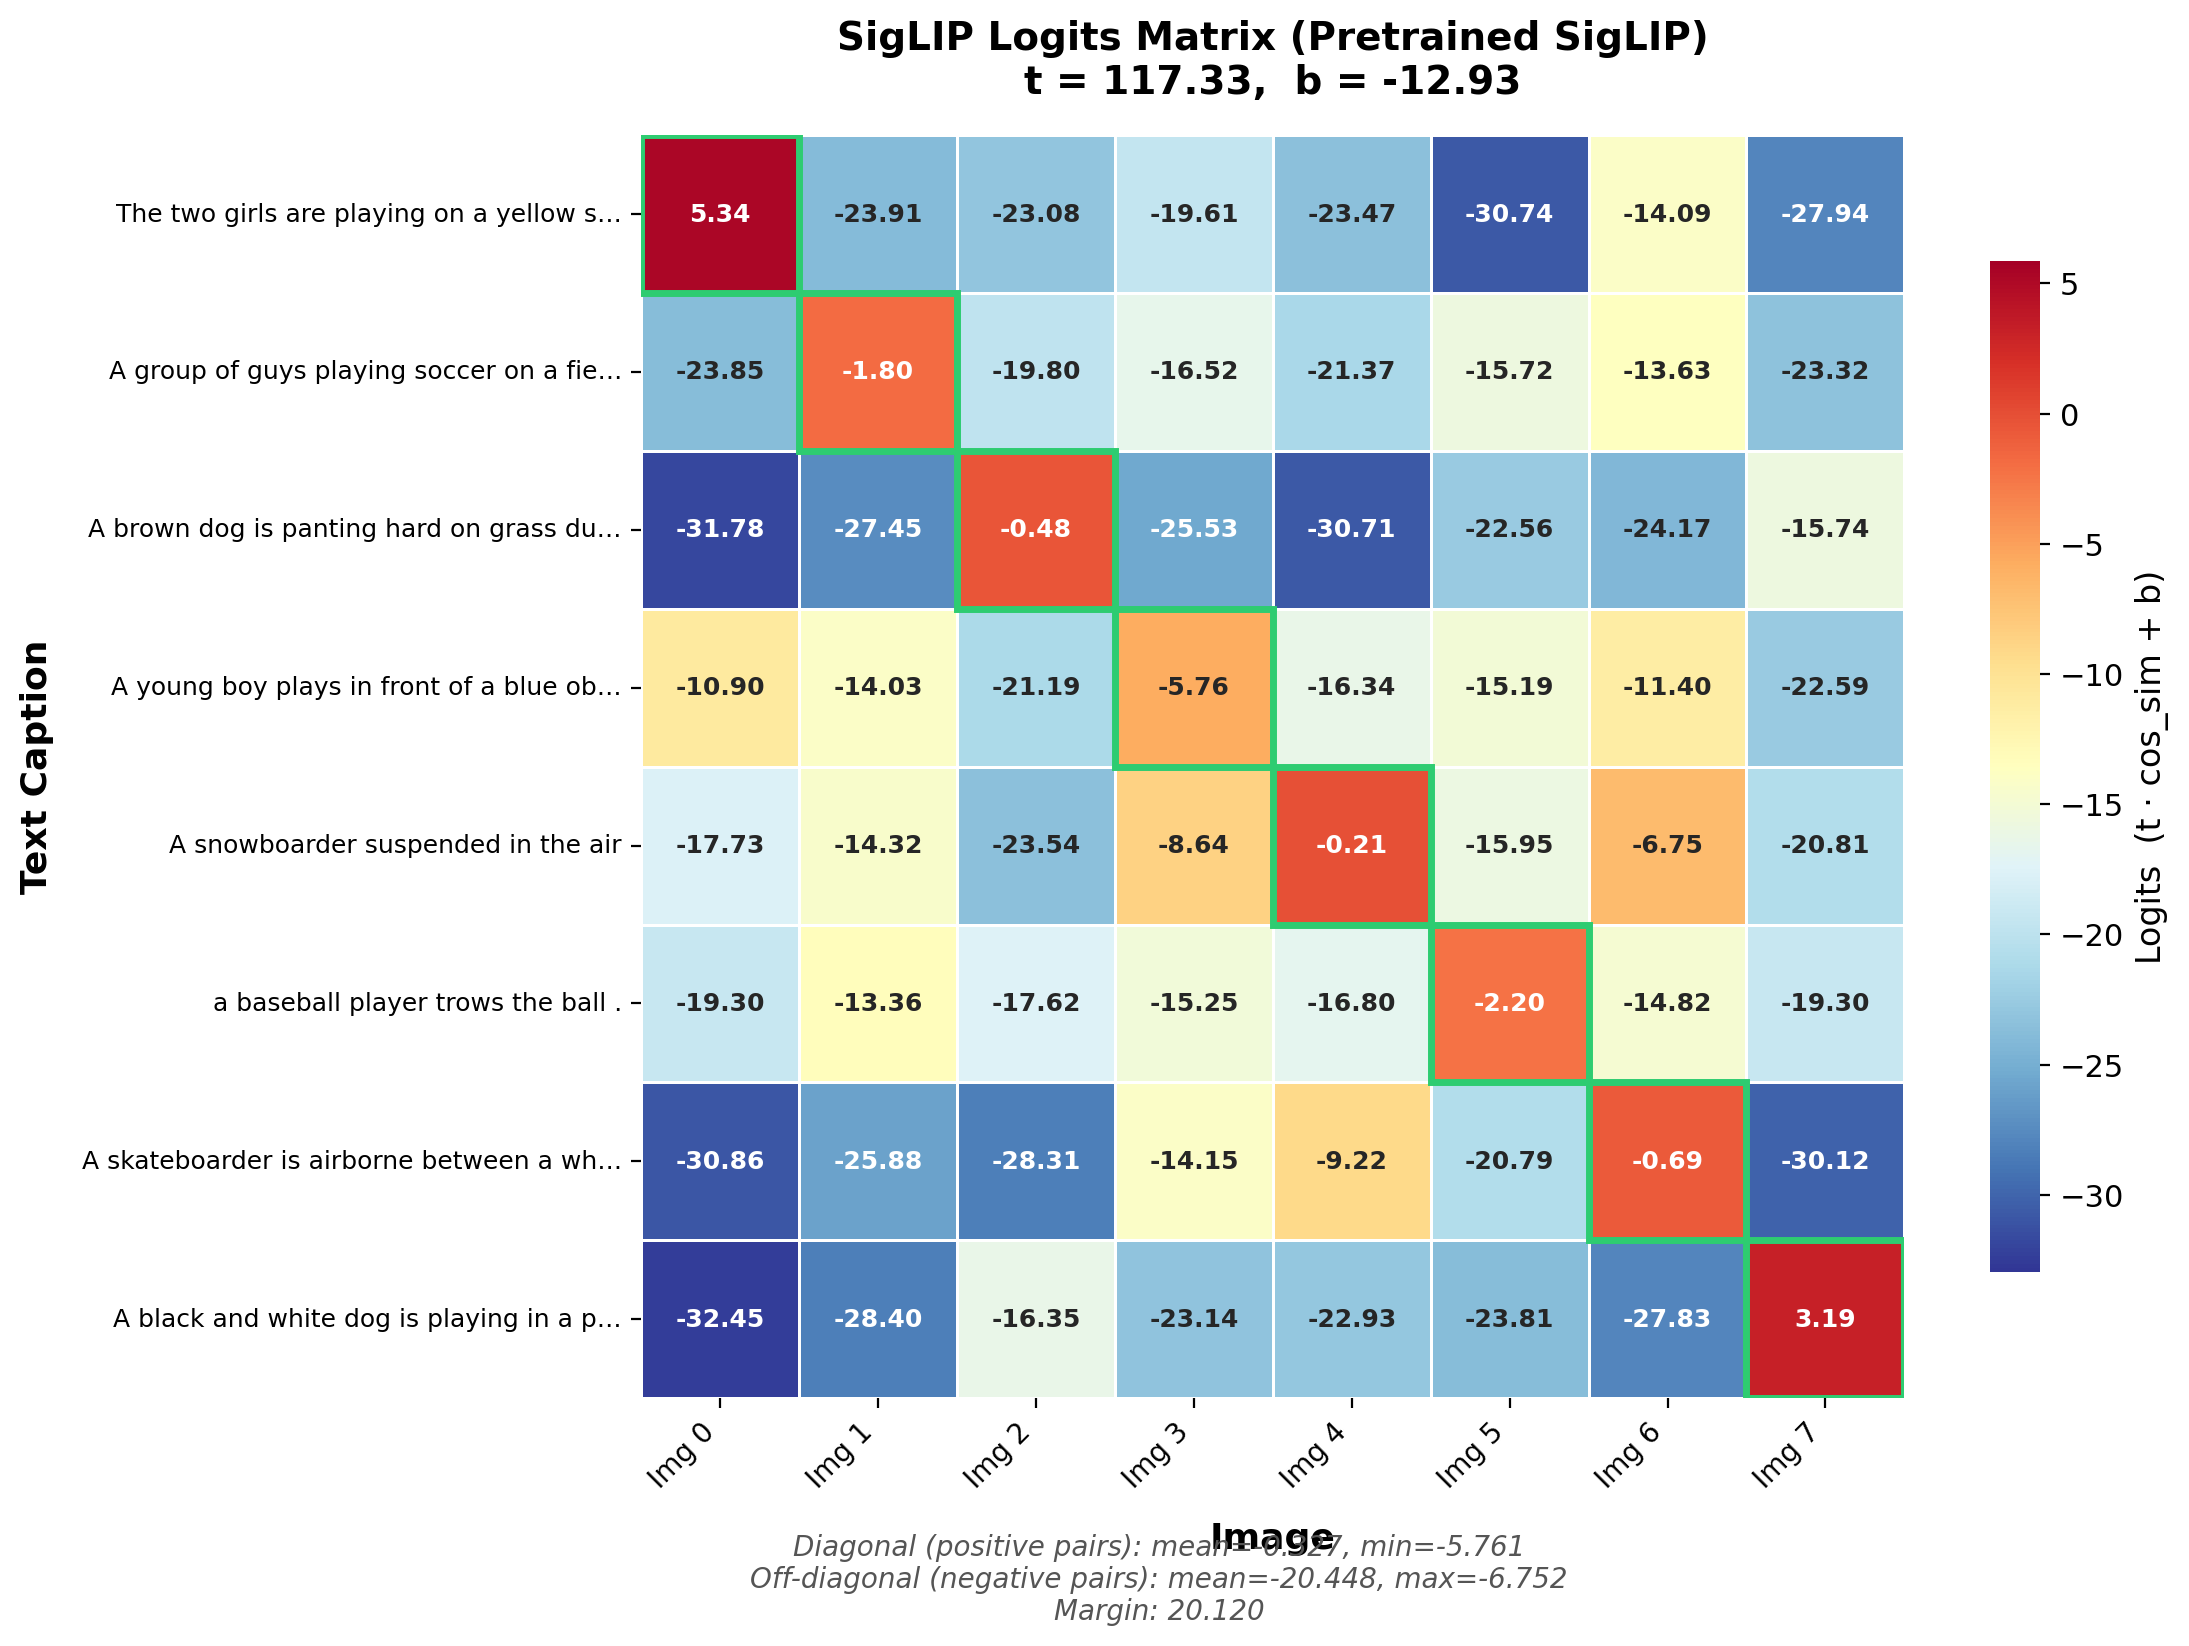
\includegraphics[width=\textwidth]{../viz_outputs/pretrained_logits_heatmap.png}
    \caption{Logits 热力图}
\end{subfigure}
\hfill
\begin{subfigure}{0.48\textwidth}
    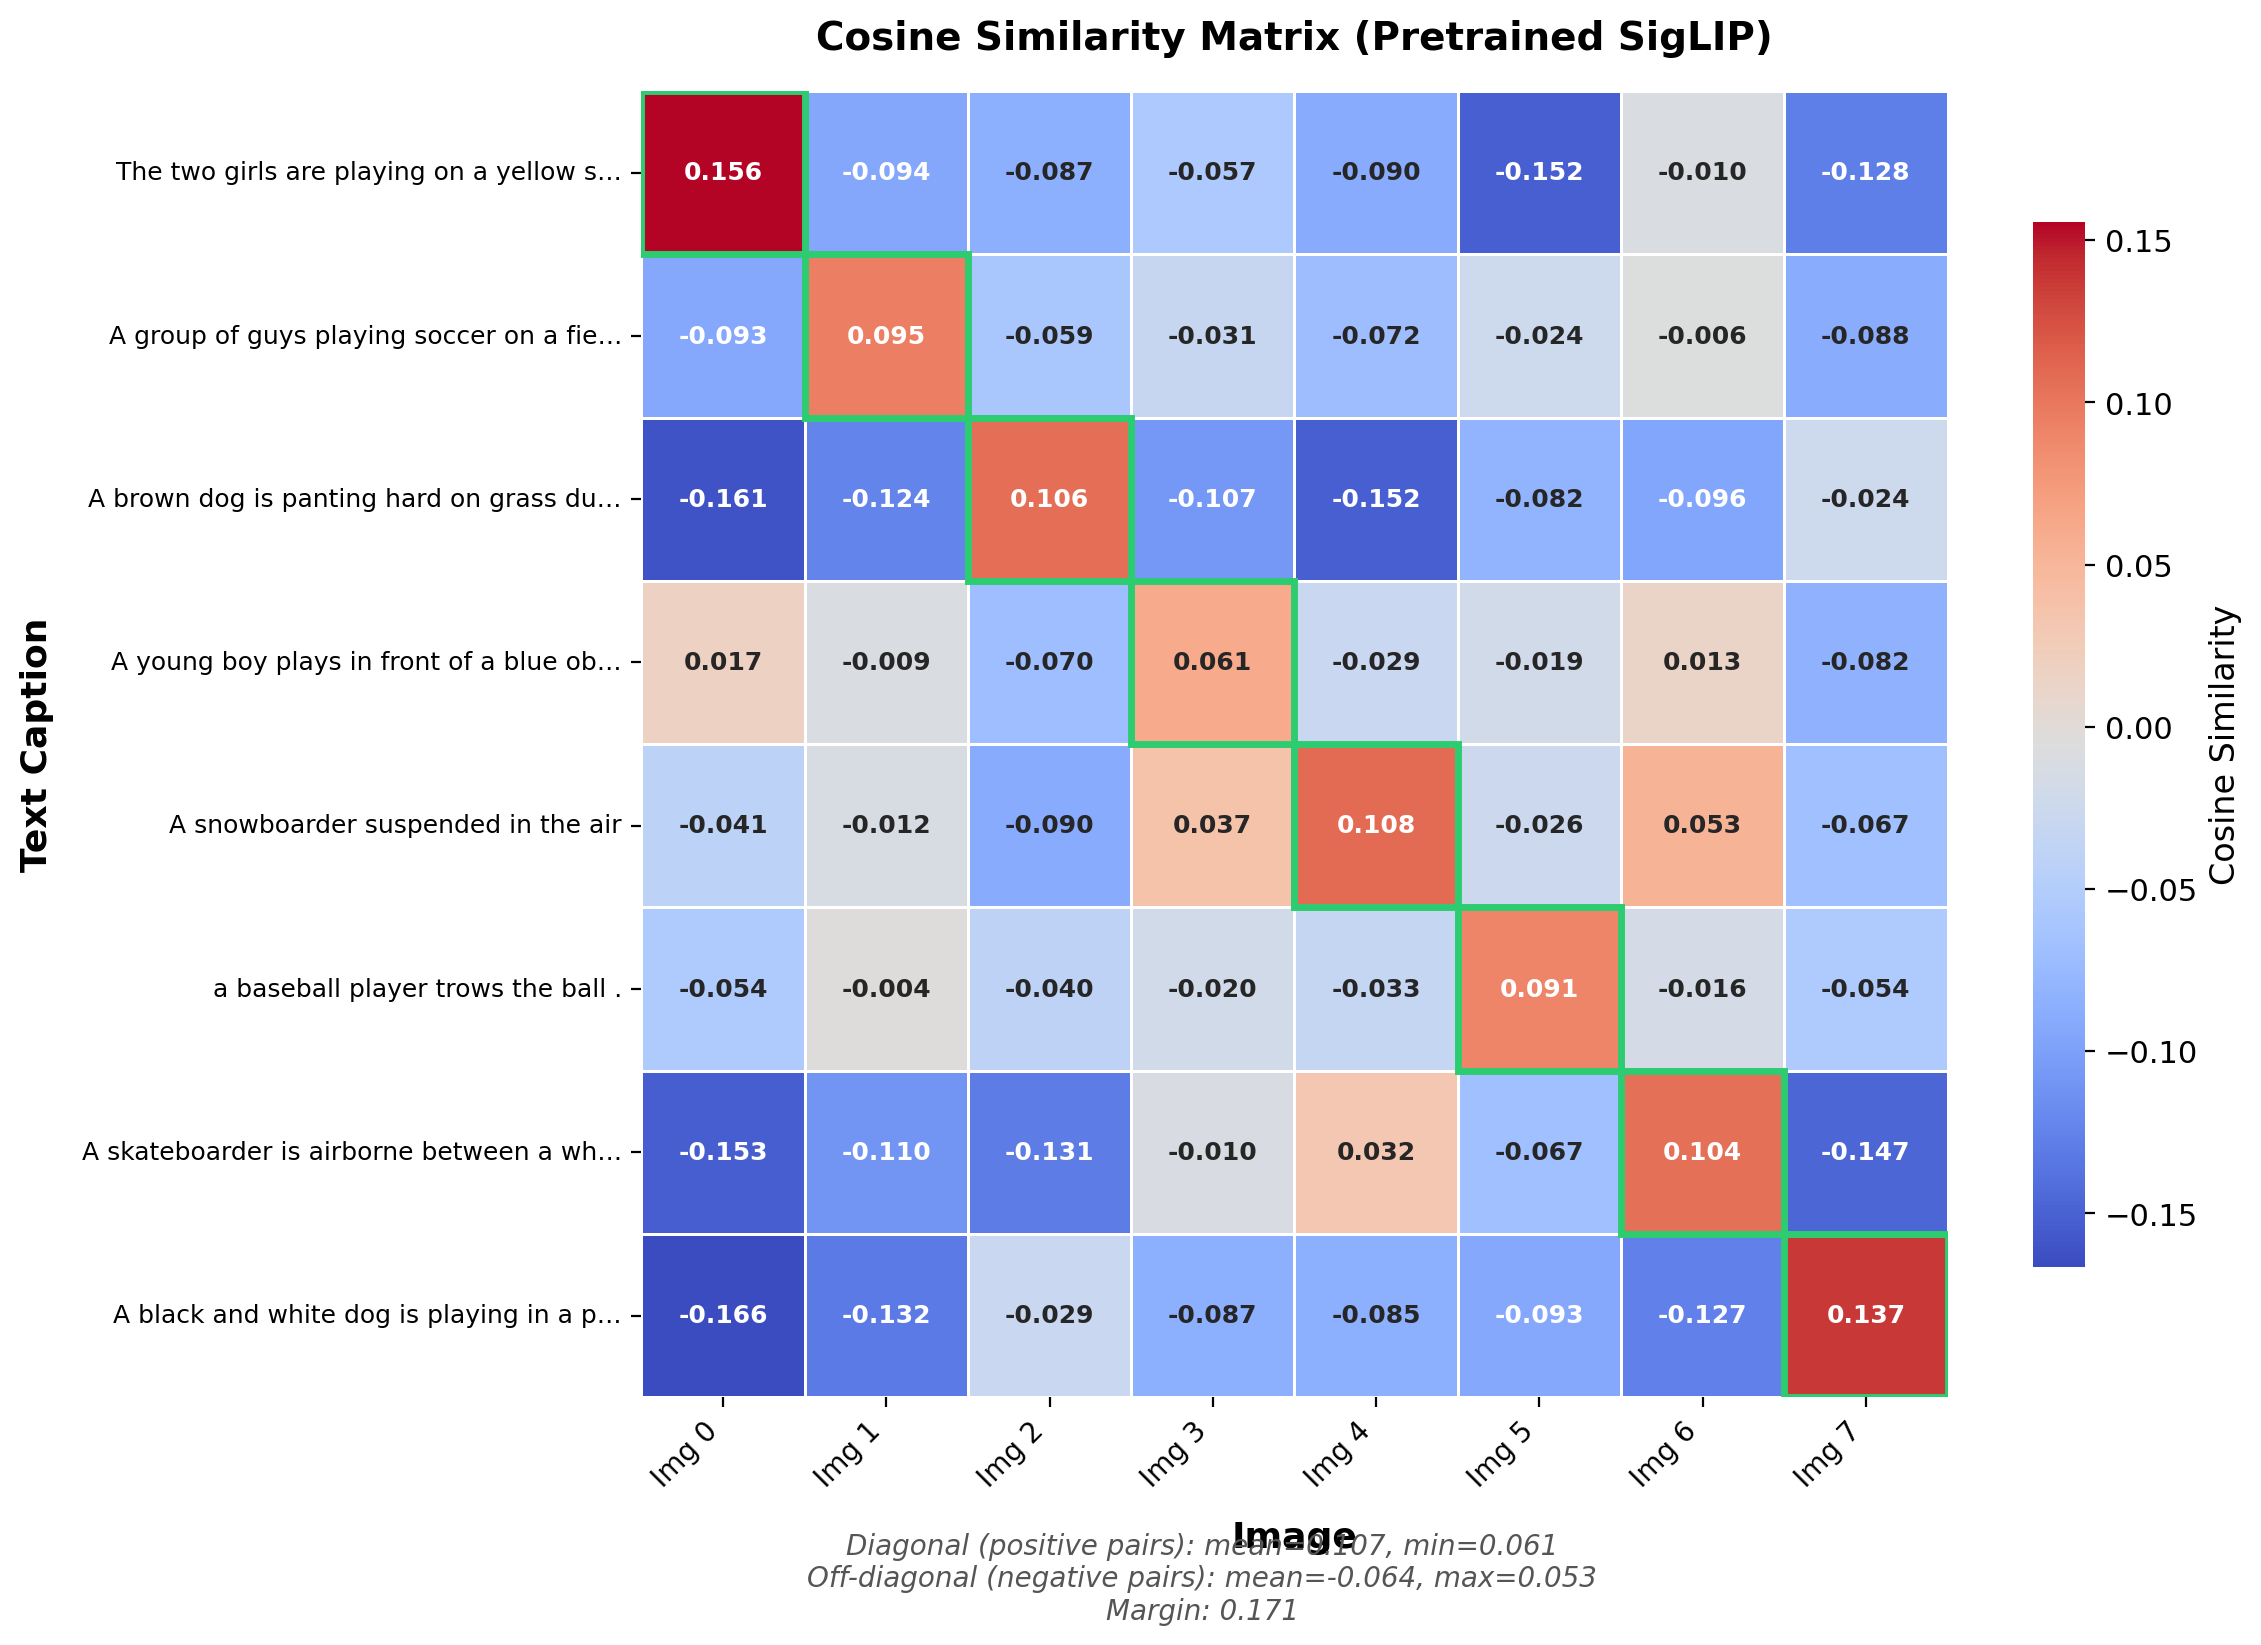
\includegraphics[width=\textwidth]{../viz_outputs/pretrained_logits_heatmap_cosine.png}
    \caption{余弦相似度热力图}
\end{subfigure}
\caption{预训练 SigLIP 模型（$t=117.33$, $b=-12.93$）}
\end{figure}

\begin{figure}[H]
\centering
\begin{subfigure}{0.48\textwidth}
    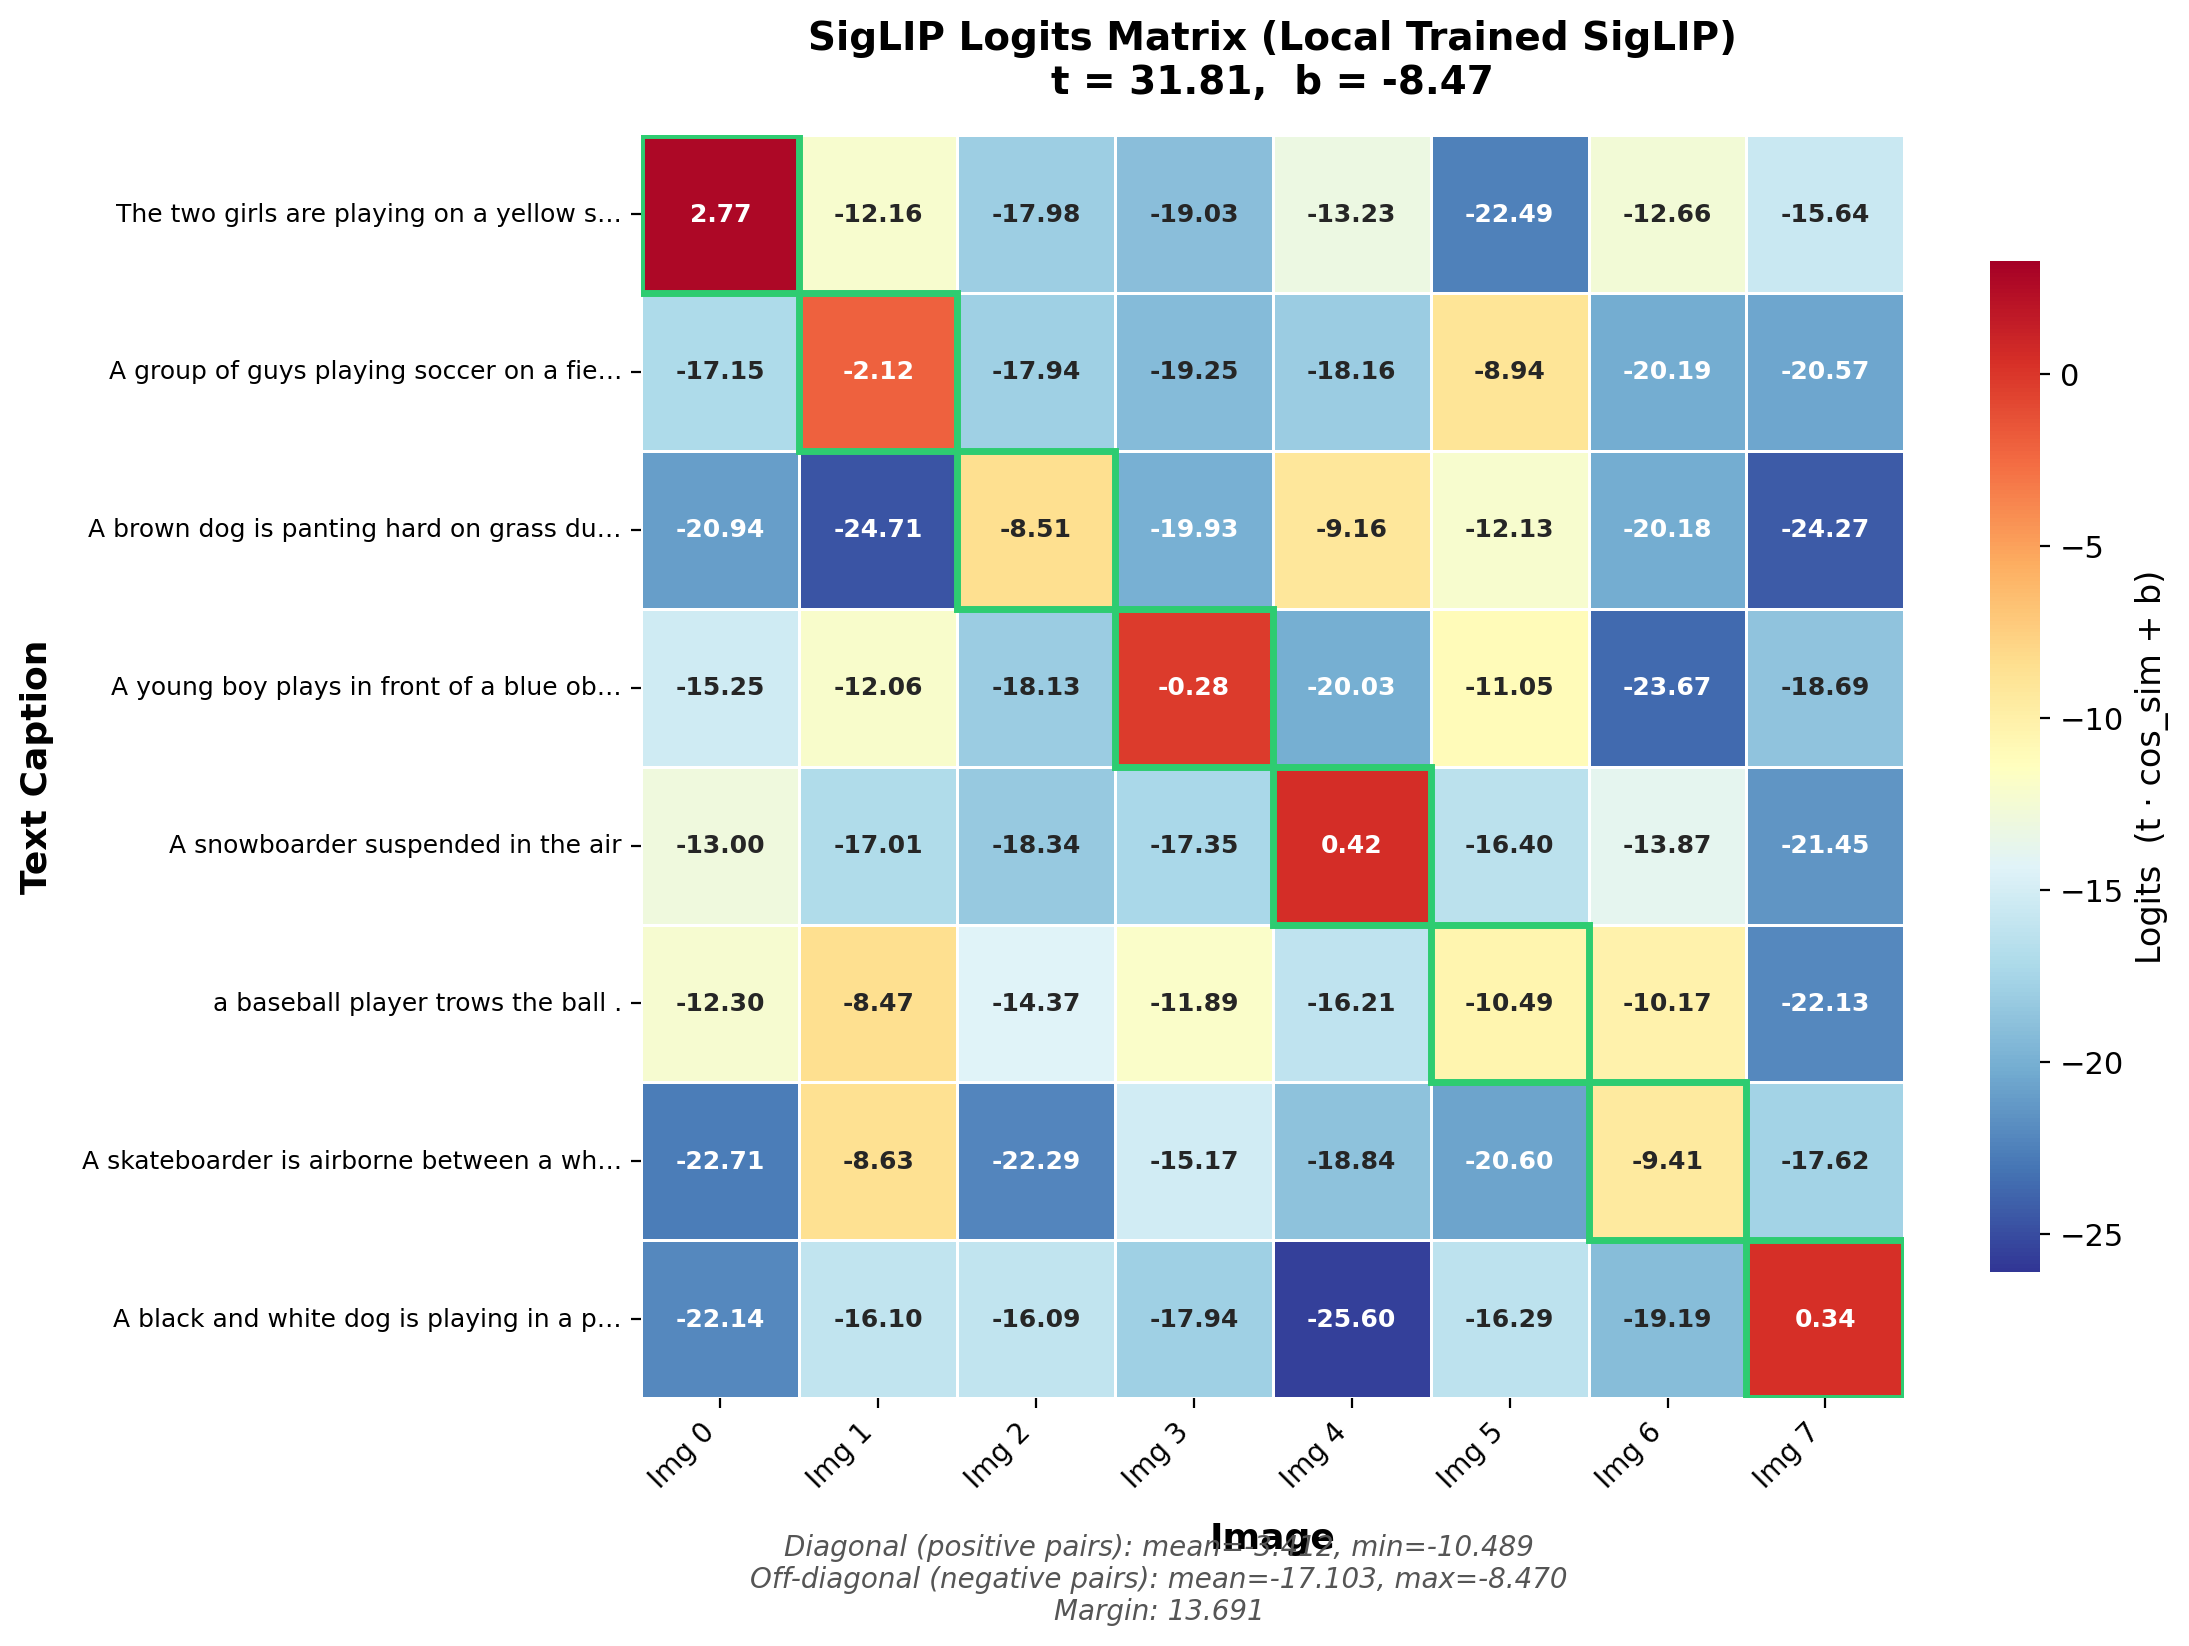
\includegraphics[width=\textwidth]{../viz_outputs/local_logits_heatmap.png}
    \caption{Logits 热力图}
\end{subfigure}
\hfill
\begin{subfigure}{0.48\textwidth}
    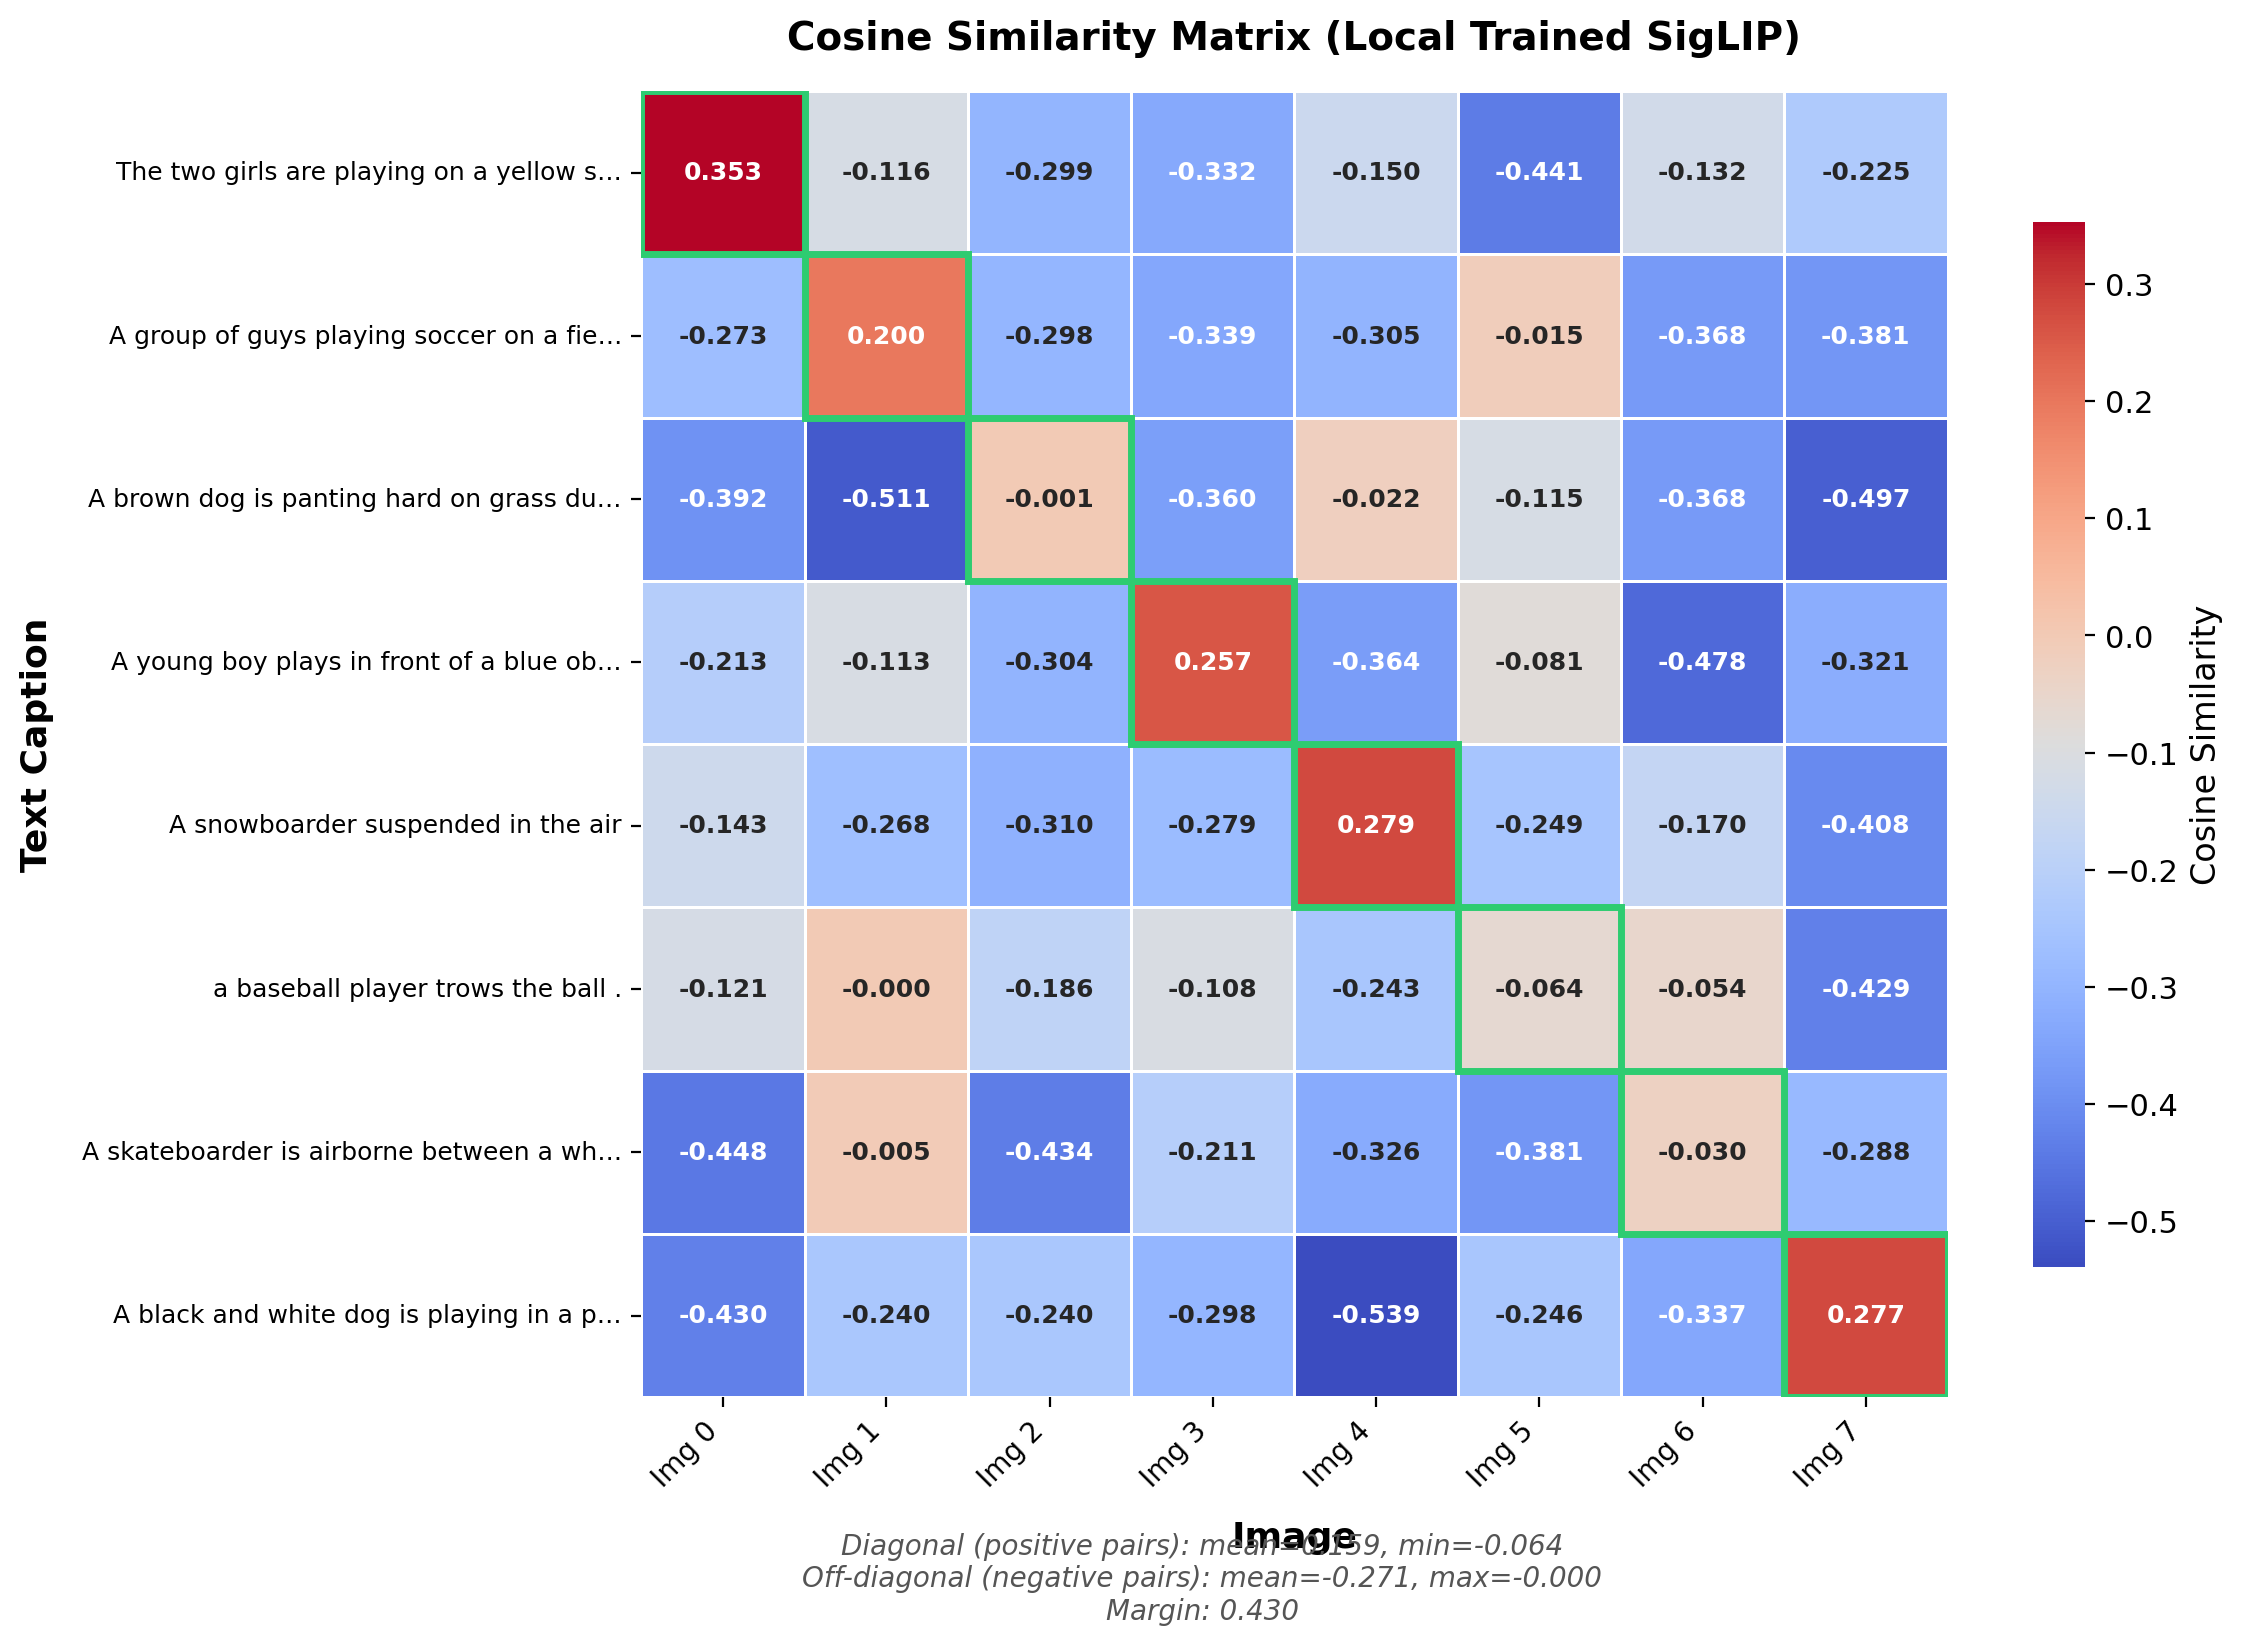
\includegraphics[width=\textwidth]{../viz_outputs/local_logits_heatmap_cosine.png}
    \caption{余弦相似度热力图}
\end{subfigure}
\caption{本地训练 SigLIP 模型（$t=31.81$, $b=-8.47$）}
\end{figure}

\textbf{对比分析}：

\begin{enumerate}[nosep]
    \item \textbf{对角线 vs 非对角线}：两个模型的对角线（正样本对）均明显高于非对角线（负样本对），说明模型成功学习到了图文对齐能力。
    \item \textbf{预训练模型优势}：预训练模型的余弦相似度对角线值更高（约 0.35--0.45），非对角线更低（约 0.05--0.15），正负对比更鲜明。这得益于 ViT 图像编码器和大规模预训练。
    \item \textbf{本地模型的局限}：本地模型的余弦相似度分布更紧凑（对角线约 0.20--0.28，非对角线约 0.05--0.15），正负样本区分度较低，反映了小数据集训练的局限。
    \item \textbf{SigLIP 缩放效果}：两个模型通过 $\text{logits} = t \cdot \cos\_sim + b$ 缩放后，对角线与非对角线的差异被显著放大。预训练模型因 $t$ 更大（117.33 vs 31.81），logits 范围更广（约 $[-20, 40]$ vs $[-5, 15]$），sigmoid 后正负区分更明显。
\end{enumerate}

\subsection{Top-K 检索可视化}

使用本地最优模型（Exp11 checkpoint），输入查询文本 ``A little girl covered in paint sits in front of a painted rainbow''，检索 Top-5 最相似图像：

\begin{figure}[H]
\centering
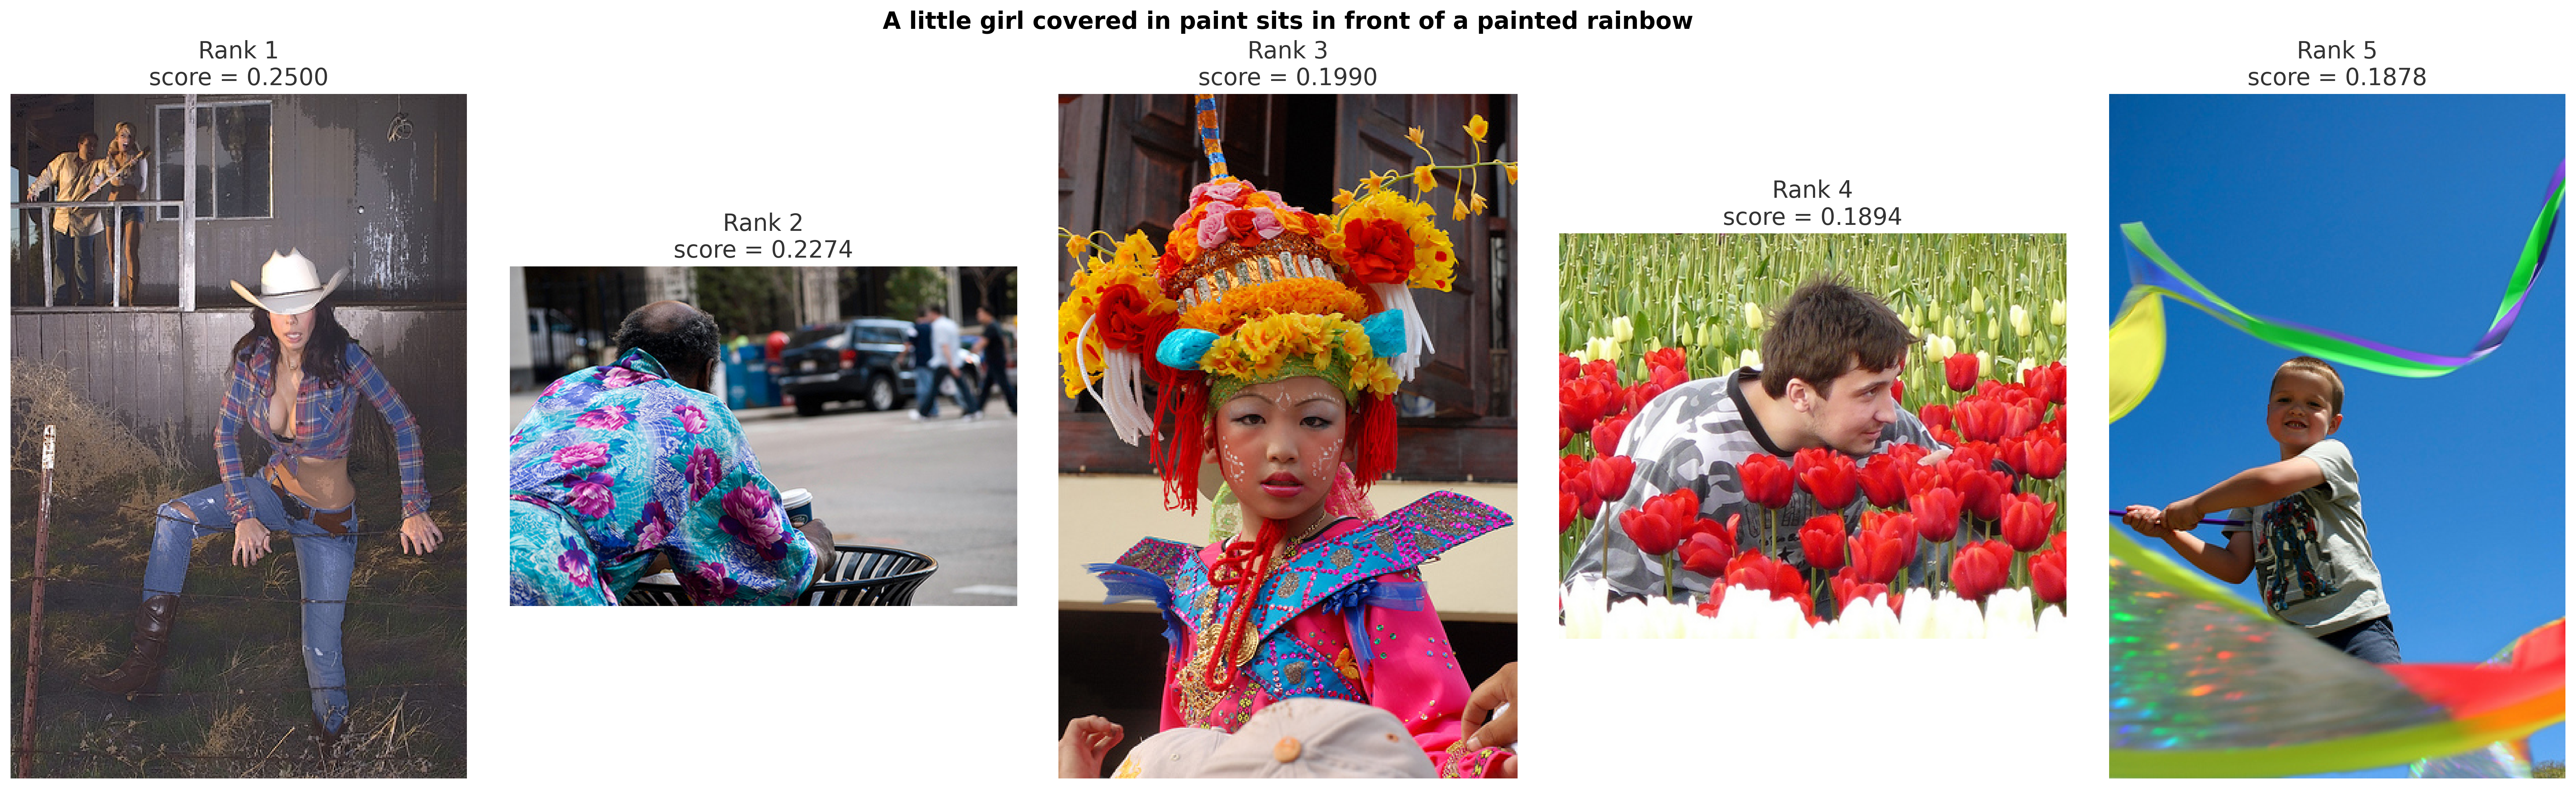
\includegraphics[width=\textwidth]{../viz_outputs/local_topk_query.png}
\caption{文本→图像 Top-5 检索结果示例}
\end{figure}

检索结果中，Rank 1 的图像确实与查询描述高度相关（涉及绘画/涂色的儿童场景），说明模型在具象描述上具有较好的检索能力。相似度分数在 0.15--0.25 范围内，整体偏低，反映了小模型嵌入空间的区分度有限。

\subsection{Bad Case 分析}

自动遍历测试集，挖掘 Ground Truth 图像排在 Top-10 之外的 Bad Case。在检索评估中，Recall@K 检查的是数据集中与 caption 配对的\textbf{原图}是否出现在 Top-K——即使检索到的其他图像语义上看似相关，只要不是那张配对的原图，仍然是检索失败。发现两类典型 Bad Case：

\begin{figure}[H]
\centering
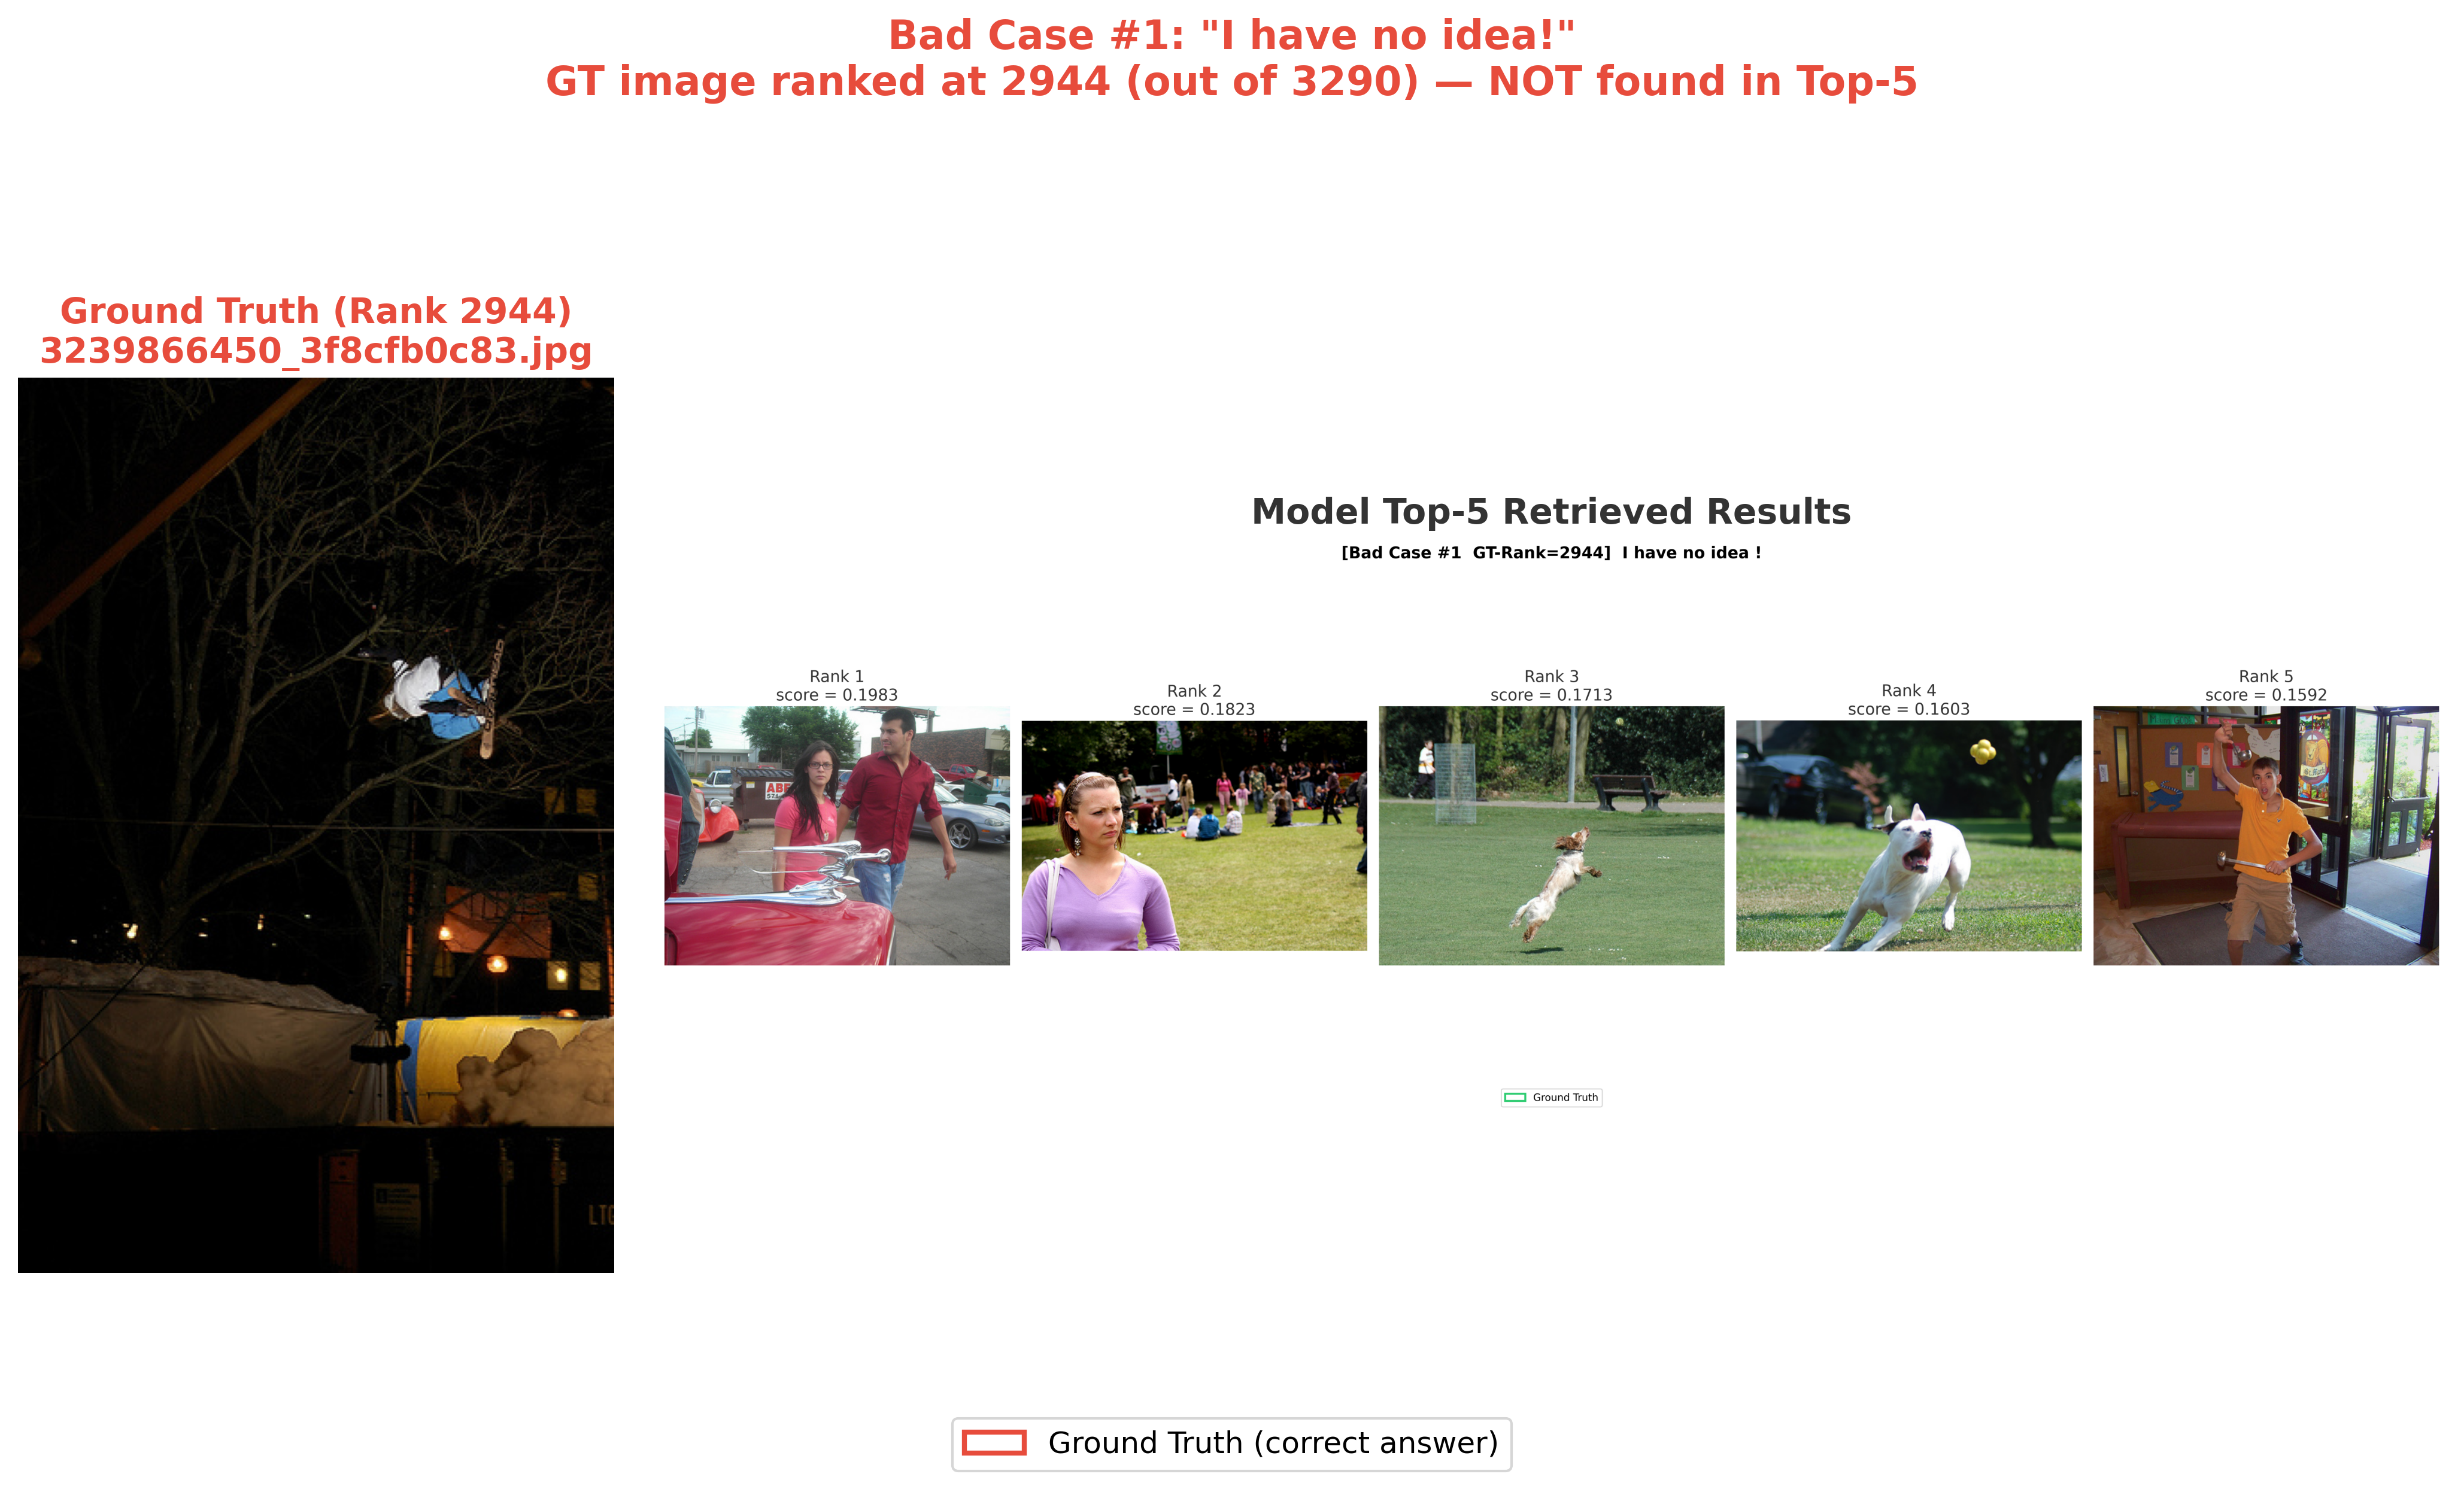
\includegraphics[width=\textwidth]{../viz_outputs/badcase1_comparison.png}
\caption{Bad Case \#1 对比：左边红框为 GT 原图（rank=2944），右边为模型 Top-5 检索结果——模型完全无法将模糊描述 ``I have no idea!'' 与任何特定图像对齐}
\end{figure}

\begin{figure}[H]
\centering
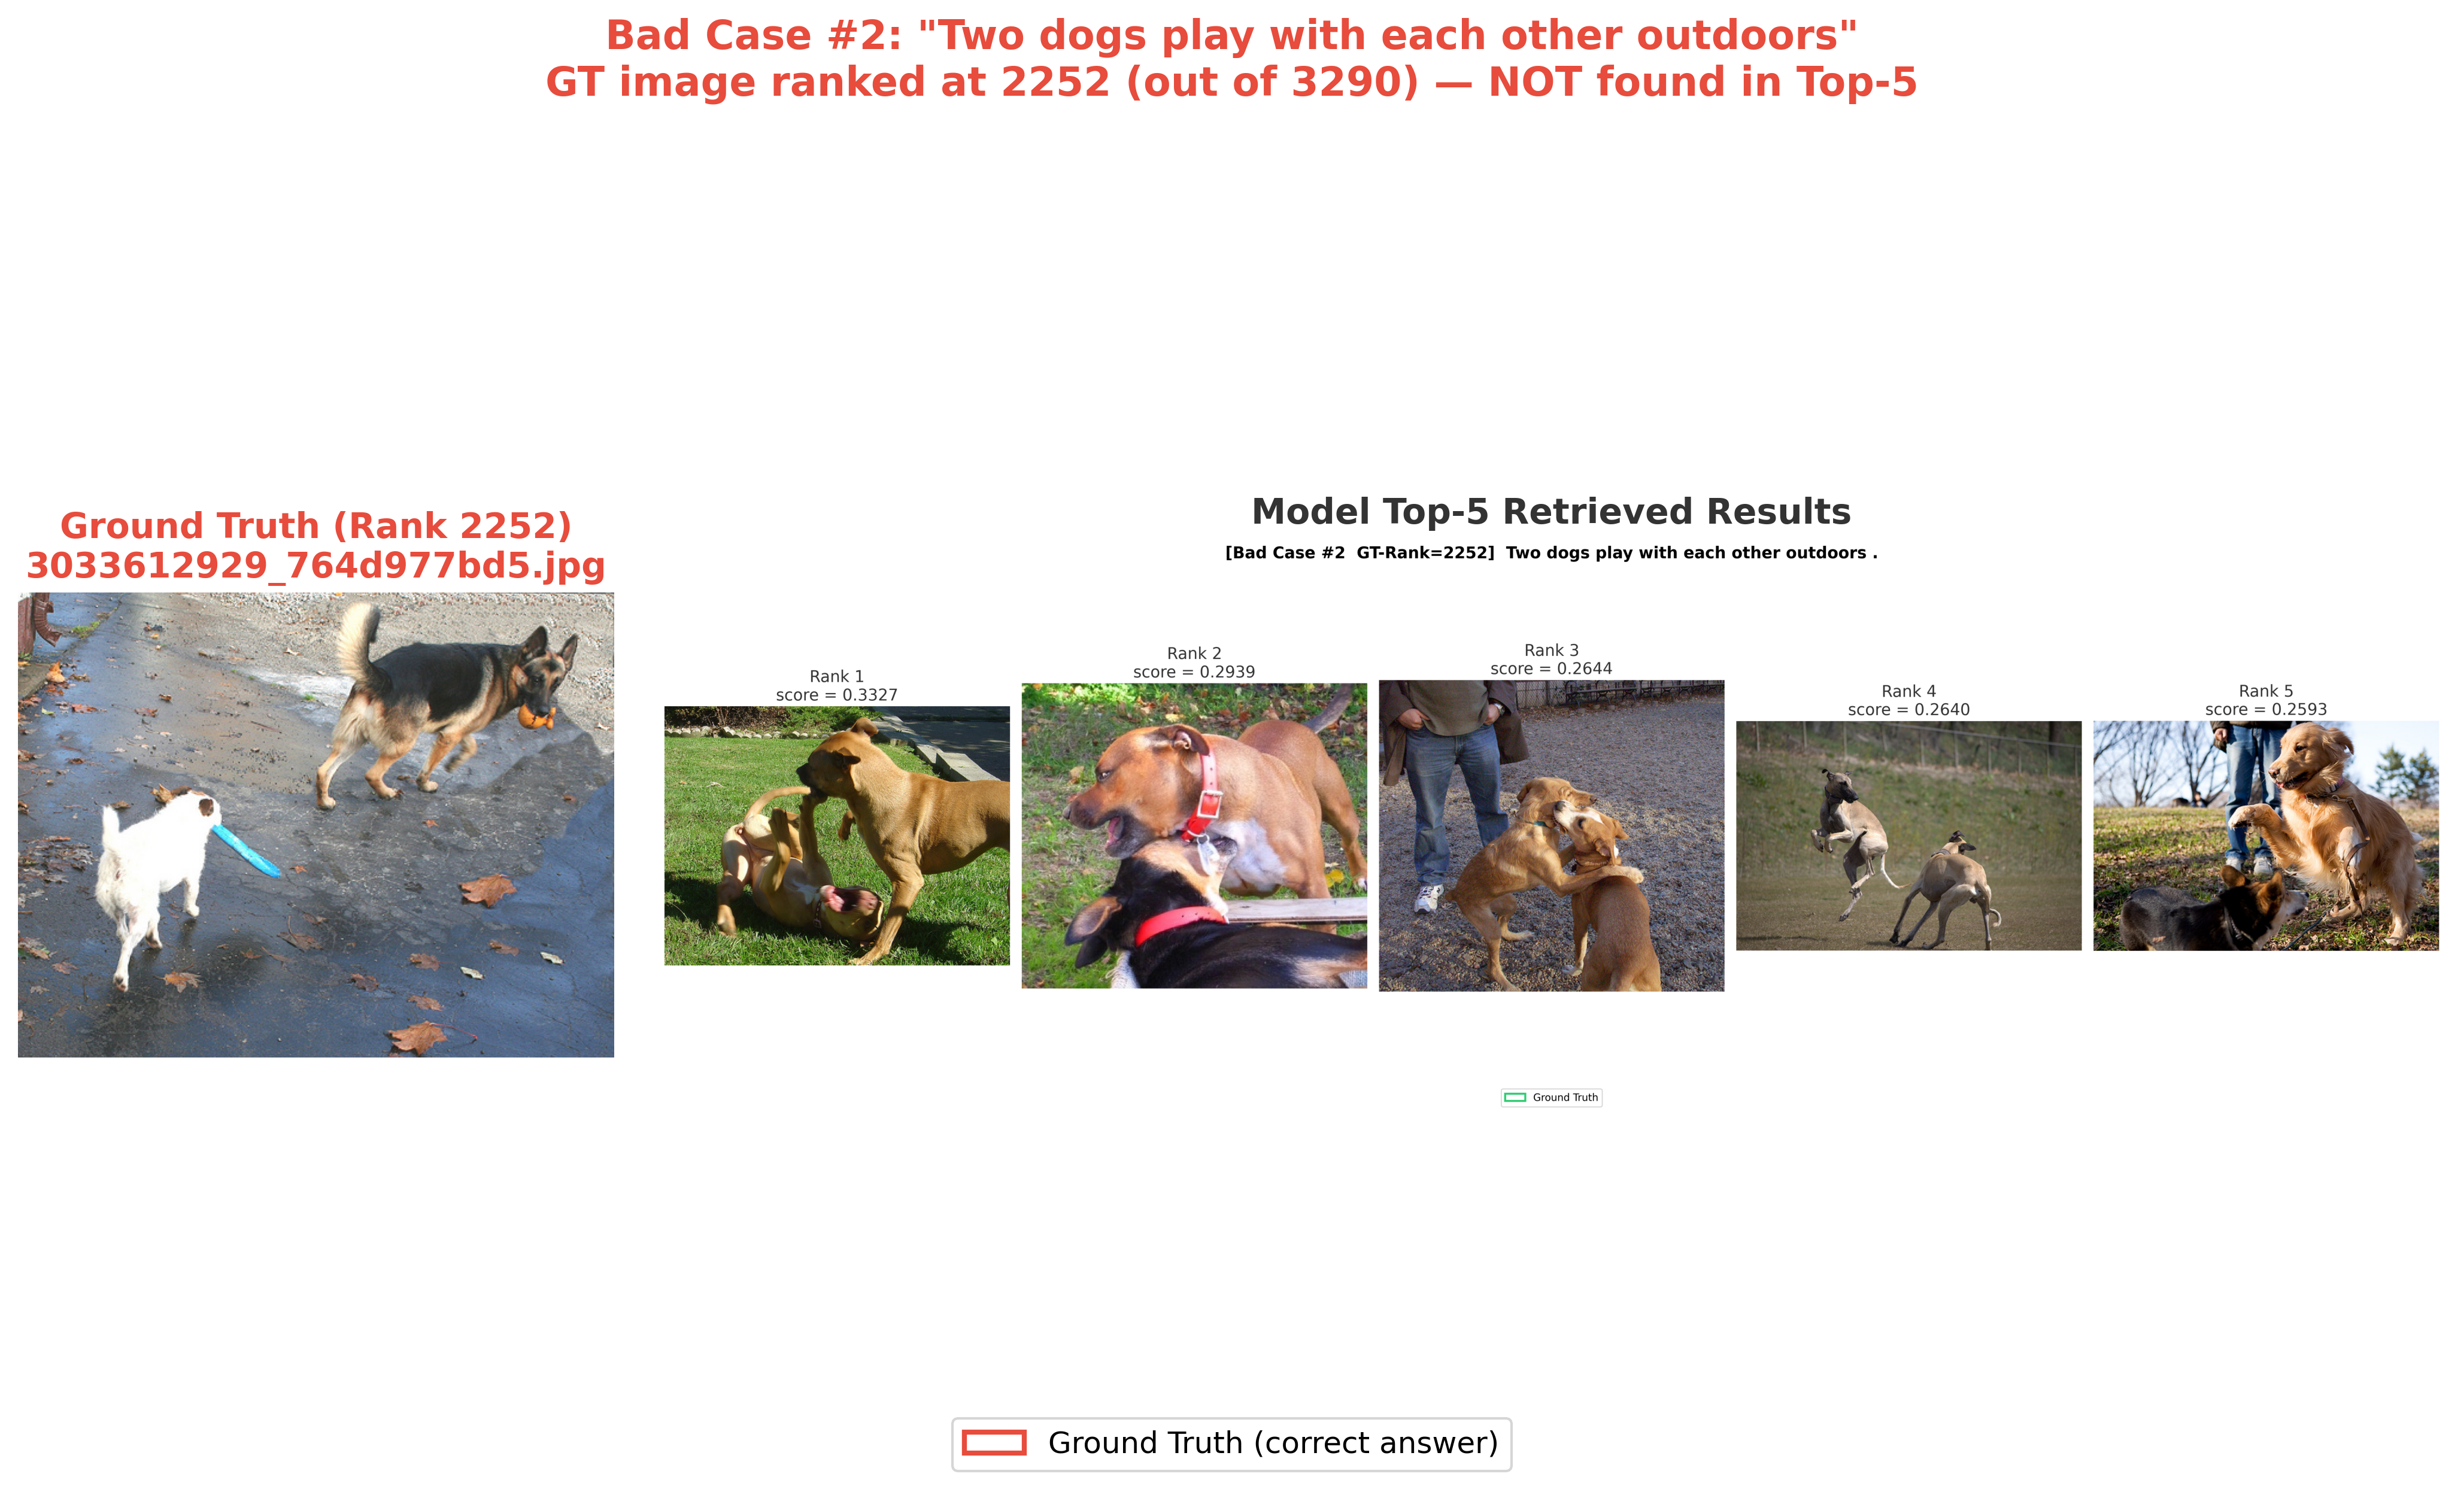
\includegraphics[width=\textwidth]{../viz_outputs/badcase2_comparison.png}
\caption{Bad Case \#2 对比：左边红框为 GT 原图（rank=2252），右边为模型 Top-5 检索结果——5 张图语义上确实都是两只狗在户外玩耍，但均非数据集中配对的原图}
\end{figure}

\textbf{Bad Case 类型分析}：

\begin{enumerate}
    \item \textbf{模糊/抽象描述}（Bad Case \#1）：描述为 ``I have no idea!...''，这类缺乏具体语义信息的文本无法提供有效的检索线索，模型难以将其与任何特定图像对齐，GT 图像排在第 2944 位。

    \item \textbf{语义正确但非精确匹配}（Bad Case \#2）：查询文本为 ``Two dogs play with each other outdoors''，GT 原图确实是两只狗在户外玩耍。模型返回的 Top-5 图像也确实都是两只狗在户外玩的场景——从语义角度来说检索是合理的。然而 Flickr8k 的评测标准要求\textbf{精确匹配数据集中配对的原图}，而非仅语义相似即可。GT 原图排在第 2252 位，说明在嵌入空间中，该配对图的相似度被大量其他"两只狗户外玩"的图像所淹没。这反映了 Flickr8k 评测的一个固有局限：当数据集中存在多张语义高度相似的图像时，Recall@K 这种精确匹配指标可能低估模型的实际语义理解能力；同时也说明小模型的嵌入空间区分度有限，无法在同一语义类别内进一步区分不同实例。
\end{enumerate}

\subsection{模型偏好与局限性总结}

综合以上可视化分析，模型表现出以下偏好和局限：

\begin{enumerate}
    \item \textbf{偏好具象、单实体描述}：模型对描述单一明确对象（如 ``a dog running on grass''）的文本检索效果较好，这类描述的关键词与图像视觉特征容易对齐。

    \item \textbf{对抽象/模糊描述薄弱}：缺乏具体语义的文本（如 ``I have no idea''）几乎无法检索到正确图像。

    \item \textbf{同类语义图像难以区分实例}：Bad Case \#2 中，模型对 ``Two dogs play outdoors'' 的 Top-5 检索结果语义上确实正确（都是两只狗户外玩），但无法精确匹配到配对原图（rank=2252）。这说明嵌入空间在同一语义类别内缺乏实例级区分能力，也反映了 Flickr8k 精确匹配评测指标的固有局限——当多张图语义高度相似时，语义正确但非精确匹配会被判为失败。

    \item \textbf{对颜色和纹理描述有一定能力}：ColorJitter 增强训练后，模型对颜色相关描述（如 ``covered in paint''）有一定检索能力，但仍不如大规模预训练模型。

    \item \textbf{整体区分度有限}：本地模型的相似度分数集中在 0.15--0.28 窄区间，与预训练模型（0.35--0.45）差距明显，这是小数据集+小模型容量的根本限制。
\end{enumerate}

%=======================================================================
\section{结论与改进方向}
%=======================================================================

\subsection{主要结论}

\begin{enumerate}[nosep]
    \item Cosine Warmup 学习率调度是最关键的优化，单独带来 8.57\% 的 t2i\_R@1 提升；
    \item ResNet width=48 + mild ColorJitter 是模型容量与泛化的最优平衡；
    \item Flickr8k 数据集对增强策略极度敏感——RandomResizedCrop、RandAugment、TrivialAugment 均严重损害性能；
    \item 更大模型容量（width=64、4L+8H+d512、MLP 投影头）在小数据集上反而导致过拟合；
    \item 最终最优模型 t2i\_R@1=36.65\%，相比中期基线提升 11.84\%。
\end{enumerate}

\subsection{改进方向}

\begin{enumerate}
    \item \textbf{使用预训练视觉编码器}：将 ResNet18 替换为 CLIP/SigLIP 的 ViT 图像编码器，利用大规模预训练的视觉特征，预计能显著提升检索准确率。

    \item \textbf{更大规模数据集}：迁移到 Flickr30k（30000 张图）或 COCO（120000 张图），对比学习需要更多负样本对提供有效训练信号。

    \item \textbf{知识蒸馏}：用预训练 SigLIP 模型的输出作为软标签，指导小模型学习更高质量的嵌入空间。

    \item \textbf{更精细的文本处理}：引入 BPE/SentencePiece 分词，扩大词表覆盖范围；增加文本编码器深度但配合更强正则化。

    \item \textbf{Hard Negative Mining}：在训练中主动挖掘模型容易混淆的负样本对，提供更有针对性的训练信号。
\end{enumerate}

%=======================================================================
\section*{附录：核心代码实现}
\addcontentsline{toc}{section}{附录：核心代码实现}
%=======================================================================

\subsection*{A.1 SigLIP 损失函数}

\begin{lstlisting}[language=Python]
class SigLIPLoss(nn.Module):
    def __init__(self, init_logit_scale=10.0, init_logit_bias=-10.0):
        super().__init__()
        self.logit_scale = nn.Parameter(torch.log(torch.tensor(init_logit_scale)))
        self.logit_bias = nn.Parameter(torch.tensor(init_logit_bias))

    def forward(self, image_embeds, text_embeds):
        image_embeds = F.normalize(image_embeds, dim=-1)
        text_embeds  = F.normalize(text_embeds, dim=-1)
        logits = image_embeds @ text_embeds.T
        t = self.logit_scale.exp()
        b = self.logit_bias
        logits = t * logits + b
        B = logits.size(0)
        labels = 2 * torch.eye(B, device=logits.device) - 1
        loss = -labels * logits
        loss = F.softplus(loss)
        return loss.sum() / B
\end{lstlisting}

\subsection*{A.2 检索评估函数}

\begin{lstlisting}[language=Python]
@torch.no_grad()
def evaluate_retrieval(model, loader, device, topk=(1, 5, 10)):
    model.eval()
    all_image_embeds, all_text_embeds = [], []
    all_image_ids, all_captions = [], []
    for batch in loader:
        images = batch["image"].to(device)
        input_ids = batch["input_ids"].to(device)
        image_embeds, text_embeds = model(images, input_ids)
        all_image_embeds.append(image_embeds)
        all_text_embeds.append(text_embeds)
        all_image_ids.extend(batch["image_id"])
        all_captions.extend(batch["caption"])
    image_embeds = F.normalize(torch.cat(all_image_embeds), dim=-1)
    text_embeds  = F.normalize(torch.cat(all_text_embeds), dim=-1)
    # 按 image_id 分组，聚合同一图像的 embedding
    img2indices = defaultdict(list)
    for idx, img_id in enumerate(all_image_ids):
        img2indices[img_id].append(idx)
    unique_images = list(img2indices.keys())
    unique_image_embeds = []
    for img_id in unique_images:
        indices = img2indices[img_id]
        unique_image_embeds.append(image_embeds[indices].mean(dim=0))
    unique_image_embeds = F.normalize(torch.stack(unique_image_embeds), dim=-1)
    sim = unique_image_embeds @ text_embeds.T
    # Text-to-Image & Image-to-Text Recall@K
    ...
\end{lstlisting}

\subsection*{A.3 可视化脚本}

项目包含两个可视化脚本：

\begin{itemize}[nosep]
    \item \texttt{visualize\_heatmap.py}：生成跨模态相似度矩阵热力图，支持预训练模型和本地模型两种模式；
    \item \texttt{visualize\_topk.py}：Top-K 检索可视化与 Bad Case 自动挖掘。
\end{itemize}

使用方法：

\begin{lstlisting}[language=bash, caption={可视化脚本使用方法}]
# 预训练模型热力图
python visualize_heatmap.py --pretrained --data-dir Flickr8k --n-pairs 8

# 本地模型热力图
python visualize_heatmap.py --checkpoint outputs/exp6/best_siglip.pt --data-dir Flickr8k

# Top-K 检索
python visualize_topk.py --checkpoint outputs/exp6/best_siglip.pt \
    --data-dir Flickr8k --caption "A dog runs through the grass" --topk 5

# Bad Case 挖掘
python visualize_topk.py --checkpoint outputs/exp6/best_siglip.pt \
    --data-dir Flickr8k --find-bad-cases --num-bad 3
\end{lstlisting}

\end{document}